\chapter{Matter and Energy}

\begin{wrapfigure}{r}{2.5in}
\noindent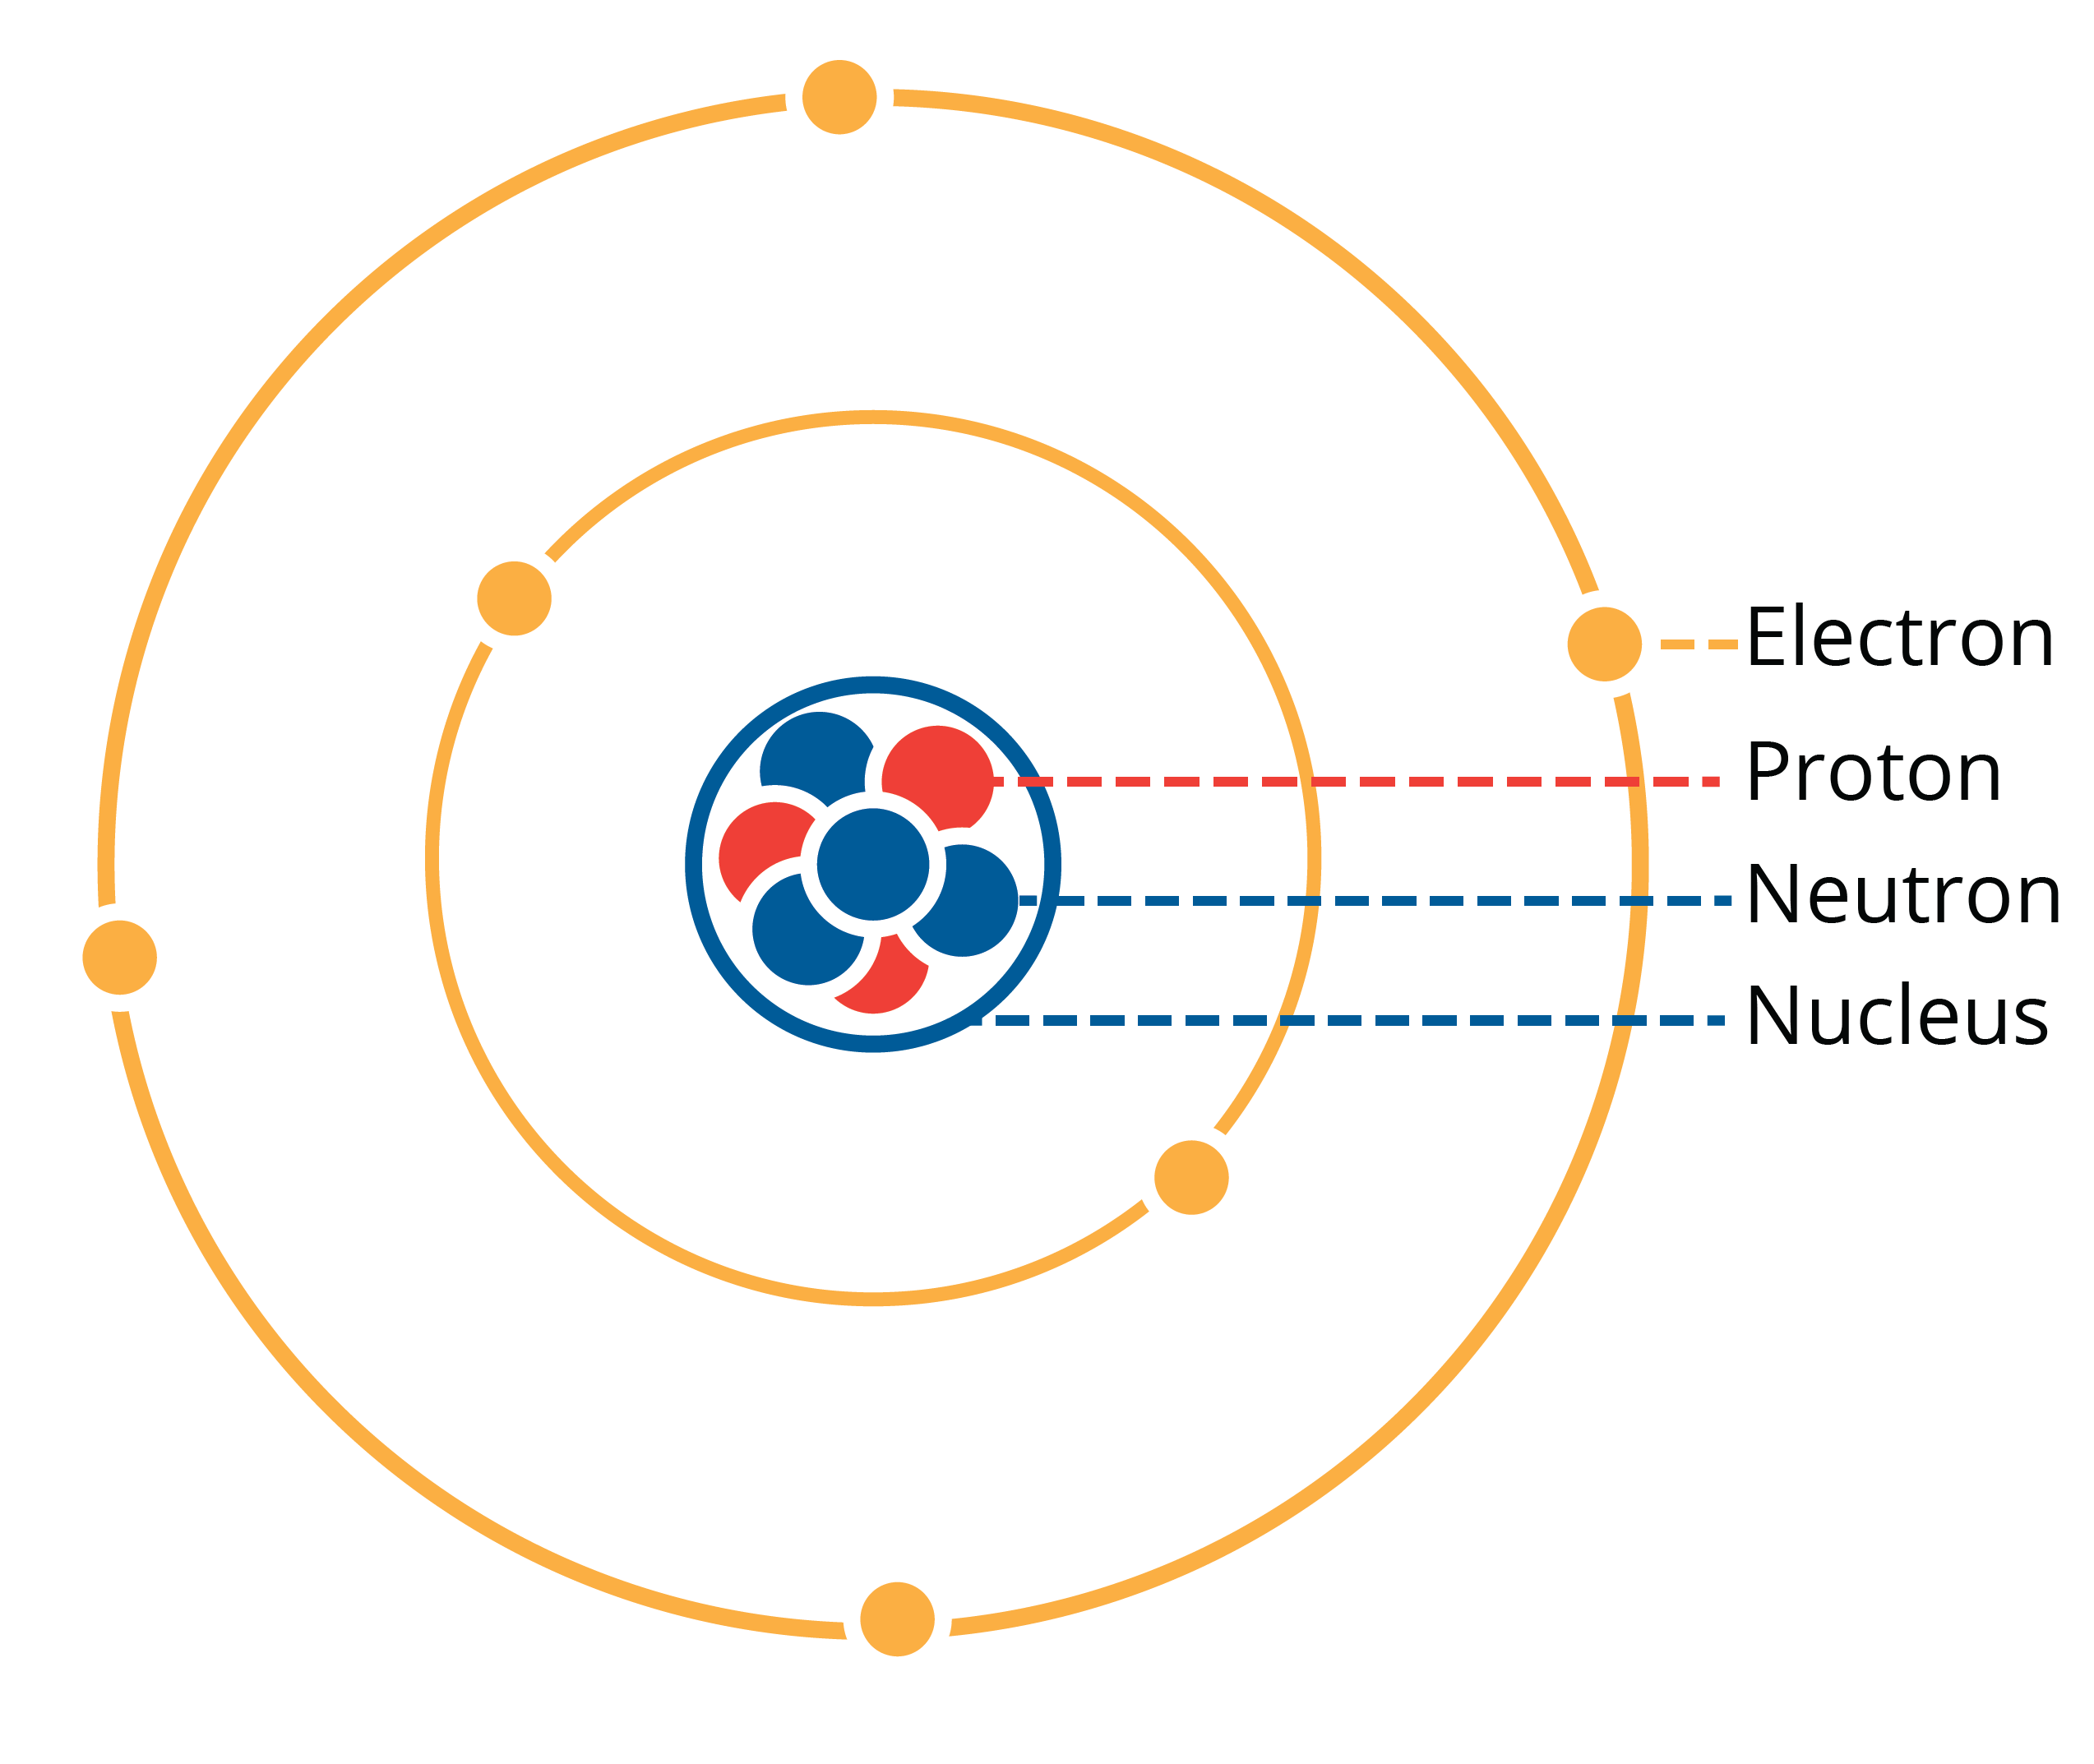
\includegraphics[trim={0 5cm 0 0}, width=2.5in]{atom1.png}
\end{wrapfigure}

All things (including the air around you) are made of atoms. Atoms are
very tiny -- there are more atoms in a drop of water than there are
drops of water in all the oceans.
% ADD: If you want a better visual of the scale: https://htwins.net/scale2/, start at around 10^-8


Every atom has a nucleus that contains protons and neutrons. Orbiting around the
nucleus is a cloud of electrons. However, the mass of the atom
comes mainly from the protons and neutrons, since they are about 2000 times as
massive as an electron.\index{protons} \index{neutrons} \index{electrons}


\subsection{Models of the Atom}
Over the history of science, there have been many ideas about the structure of
atoms. This history is a good example of how science develops: how unexpected
results drive scientists to update their models, moving us closer and closer to
a true model of the atom.

During his investigations into the behavior of gases,
John Dalton (lived 1766-1844) noted that different elements combine in strict
ratios. For example, he noted that nitrogen and oxygen combine in a 1:1 and 1:2
fashion, but no ratio in between.

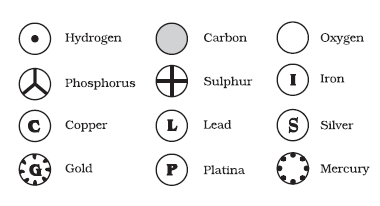
\includegraphics[width=0.75\textwidth]{daltons_model.png}

This first model of the atom is very rudimentary: each element is a unique atom,
and atoms cannot be subdivided. The atom is modeled as one large, solid, uniform,
and neutral object. Some scientists, including the British physicist J.J. Thomson
(1856-1940) thought that larger atoms (like lead) might be able to be broken down
into smaller atoms (like hydrogen). Thomson had been experimenting with cathode
ray tubes and discovered that the these rays traveled much faster than thought
possible for a particle the size of a hydrogen atom.

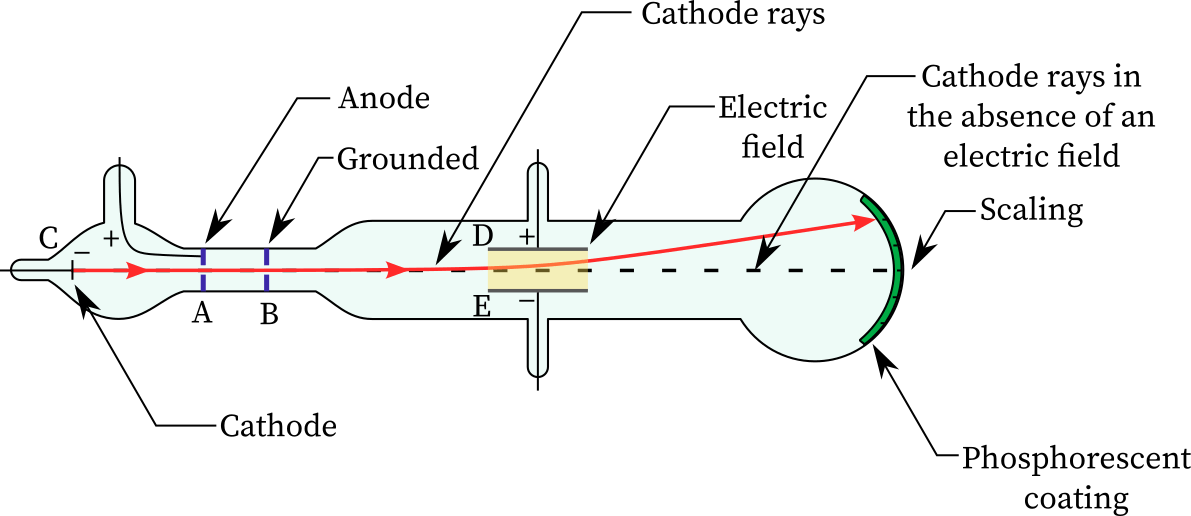
\includegraphics[width=1\textwidth]{cathode-ray-tube.png}

This, combined with the observation that cathode rays could be deflected by
electrical charge, led him to postulate two things:

\begin{enumerate}
\item Atoms can be broken into parts much smaller than a hydrogen atom
\item Whatever part of atoms that composes cathode rays is negatively charged
\end{enumerate}

\begin{wrapfigure}{l}{3in}
\noindent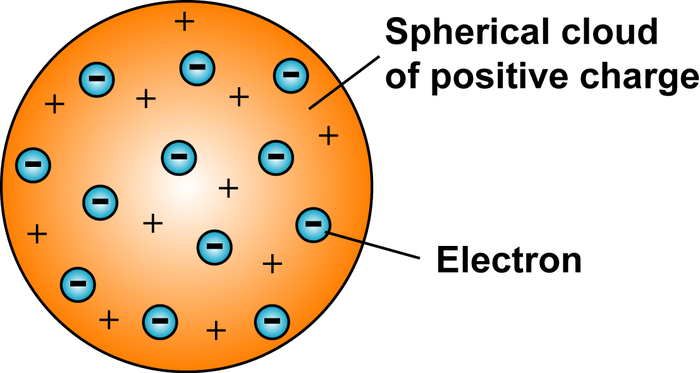
\includegraphics[width=3in]{thomson_model.png}
\end{wrapfigure}

The presence of "corpuscules" (as Thomson called them) that were negatively
charged and smaller than a hydrogen atom contradicted Dalton's theory. Thomson
updated his model of the atom: adding small, negatively charged subatomic
particles (now called electrons) that were embedded in a larger, uniform, positive
sphere. Suddenly, the atom went from neutral and indivisible to made of different
types of charged particles.

At the time, physicists were very interested in the mass-to-charge ratios of
various particles (Thomson was able to determine the mass-to-charge ratio of the
electron during his experiments), and Ernest Rutherford (1871-1937) was
investigating the mass-to-charge ratio of alpha particles. (Alpha particles, we
now know, are composed of two protons and two neutrons. They are emitted from
certain radioactive elements, including uranium.) Rutherford needed consistent
scattering of alpha particles in order to collect the data necessary to determine
the particles' mass-to-charge ratio. He achieved this by bombarding extremely
thin gold foil with alpha particles. The Thomson model of the atom would predict
that particles would be slightly deflected, as illustrated below:

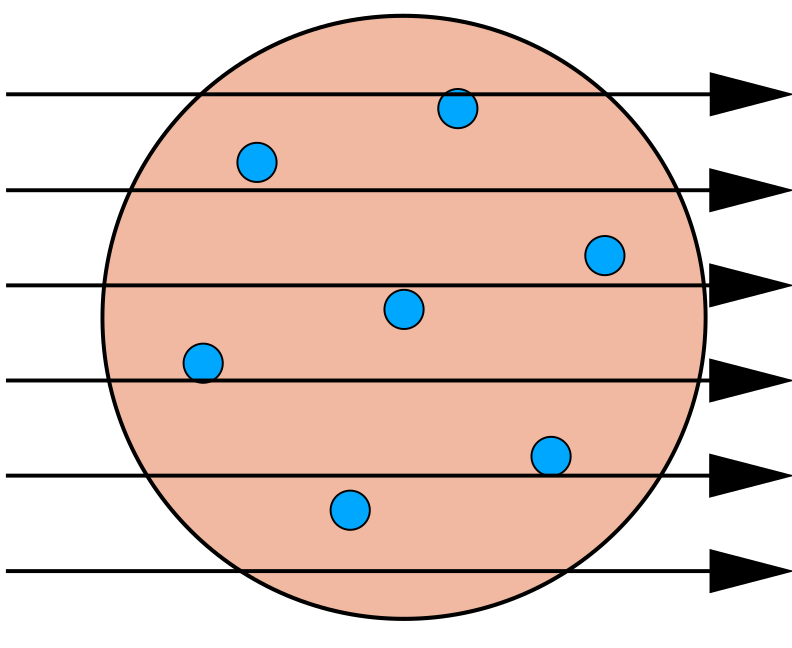
\includegraphics[width=3in]{thomson_gold.png}

However, a small but significant portion of the alpha particles were deflected
over $90 \deg$! To explain this, Rutherford modeled the atom as mostly empty
space with a small, dense, positive center (we now call this the nucleus).

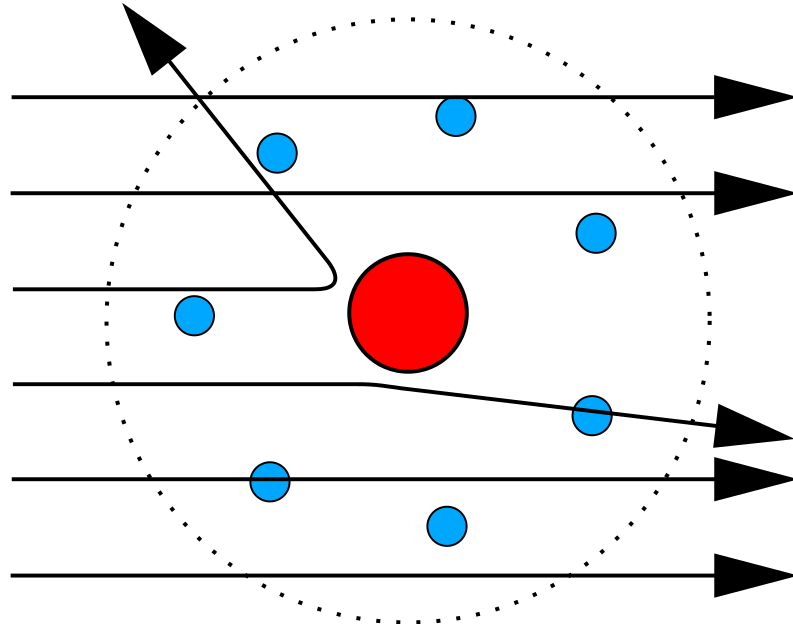
\includegraphics[width=3in]{rutherford_gold.png}


At the same time that Rutherford was conducting his gold foil experiments, Niels
Bohr was investigating the hydrogen line series. FIXME insert figure of hydrogen
lines. When hydrogen is electrically excited, it emits specific bands of color,
not a complete spectrum. Every element has a unique emission spectrum.

\noindent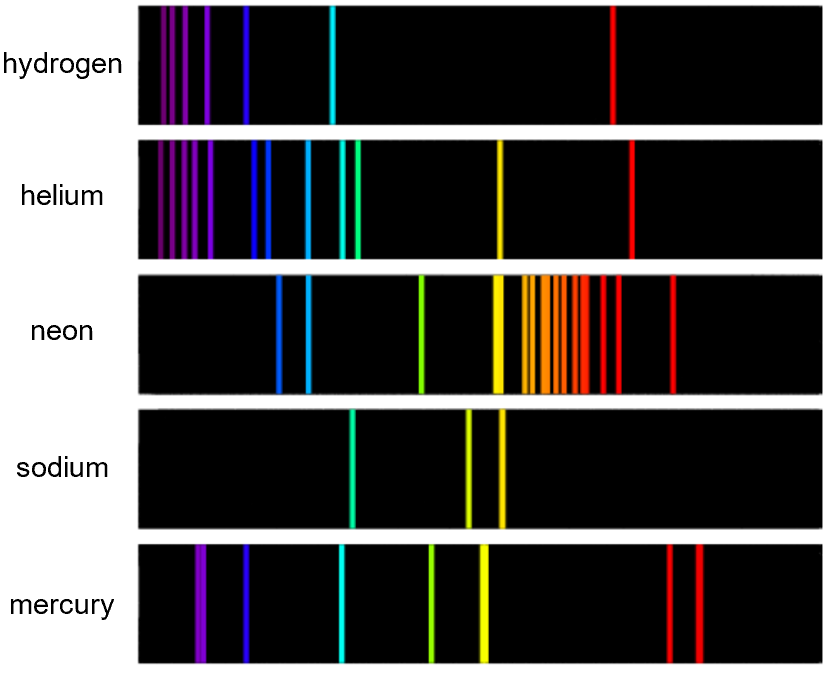
\includegraphics[width=3in]{spectral_lines.png}


Bohr, upon learning of Rutherford's experiments,
embraced the Rutherford model over the Thomson model and postulated that electrons
existed only at discrete distances from the nucleus. When electrified, a hydrogen
atom's electrons would gain energy and "jump" up one or more levels. The electron
would be unstable in this energized state, and eventually "fall" back to the
lowest energy level, emitting the extra energy as light. different colors of
light have different energies: violet being the most energetic and red being the
least. The different levels had differing amounts of energy between them,
resulting in only those colors corresponding to the exact energy step between
levels being emitted. This model, called the Bohr model or the Rutherford-Bohr
model, expands on the Rutherford model by limiting electrons to specific
distances from the nucleus, and is often compared to a model of the solar system
FIXME add image of Bohr model.

This is likely the model you are most familiar with seeing, and it is the one we
will use often in this text.


The previous graphic is slightly untrue. While it is a convenient model for
thinking about atoms, in reality electrons don't neatly orbit the nucleus.
Scientists don't know exactly where an electron will be in relation to the
nucleus, but they do know where it's most likely to be. They use a cloud that is
thicker in the center but fades out at the edges to represent an electron's
position.


\begin{wrapfigure}{l}{3in}
\noindent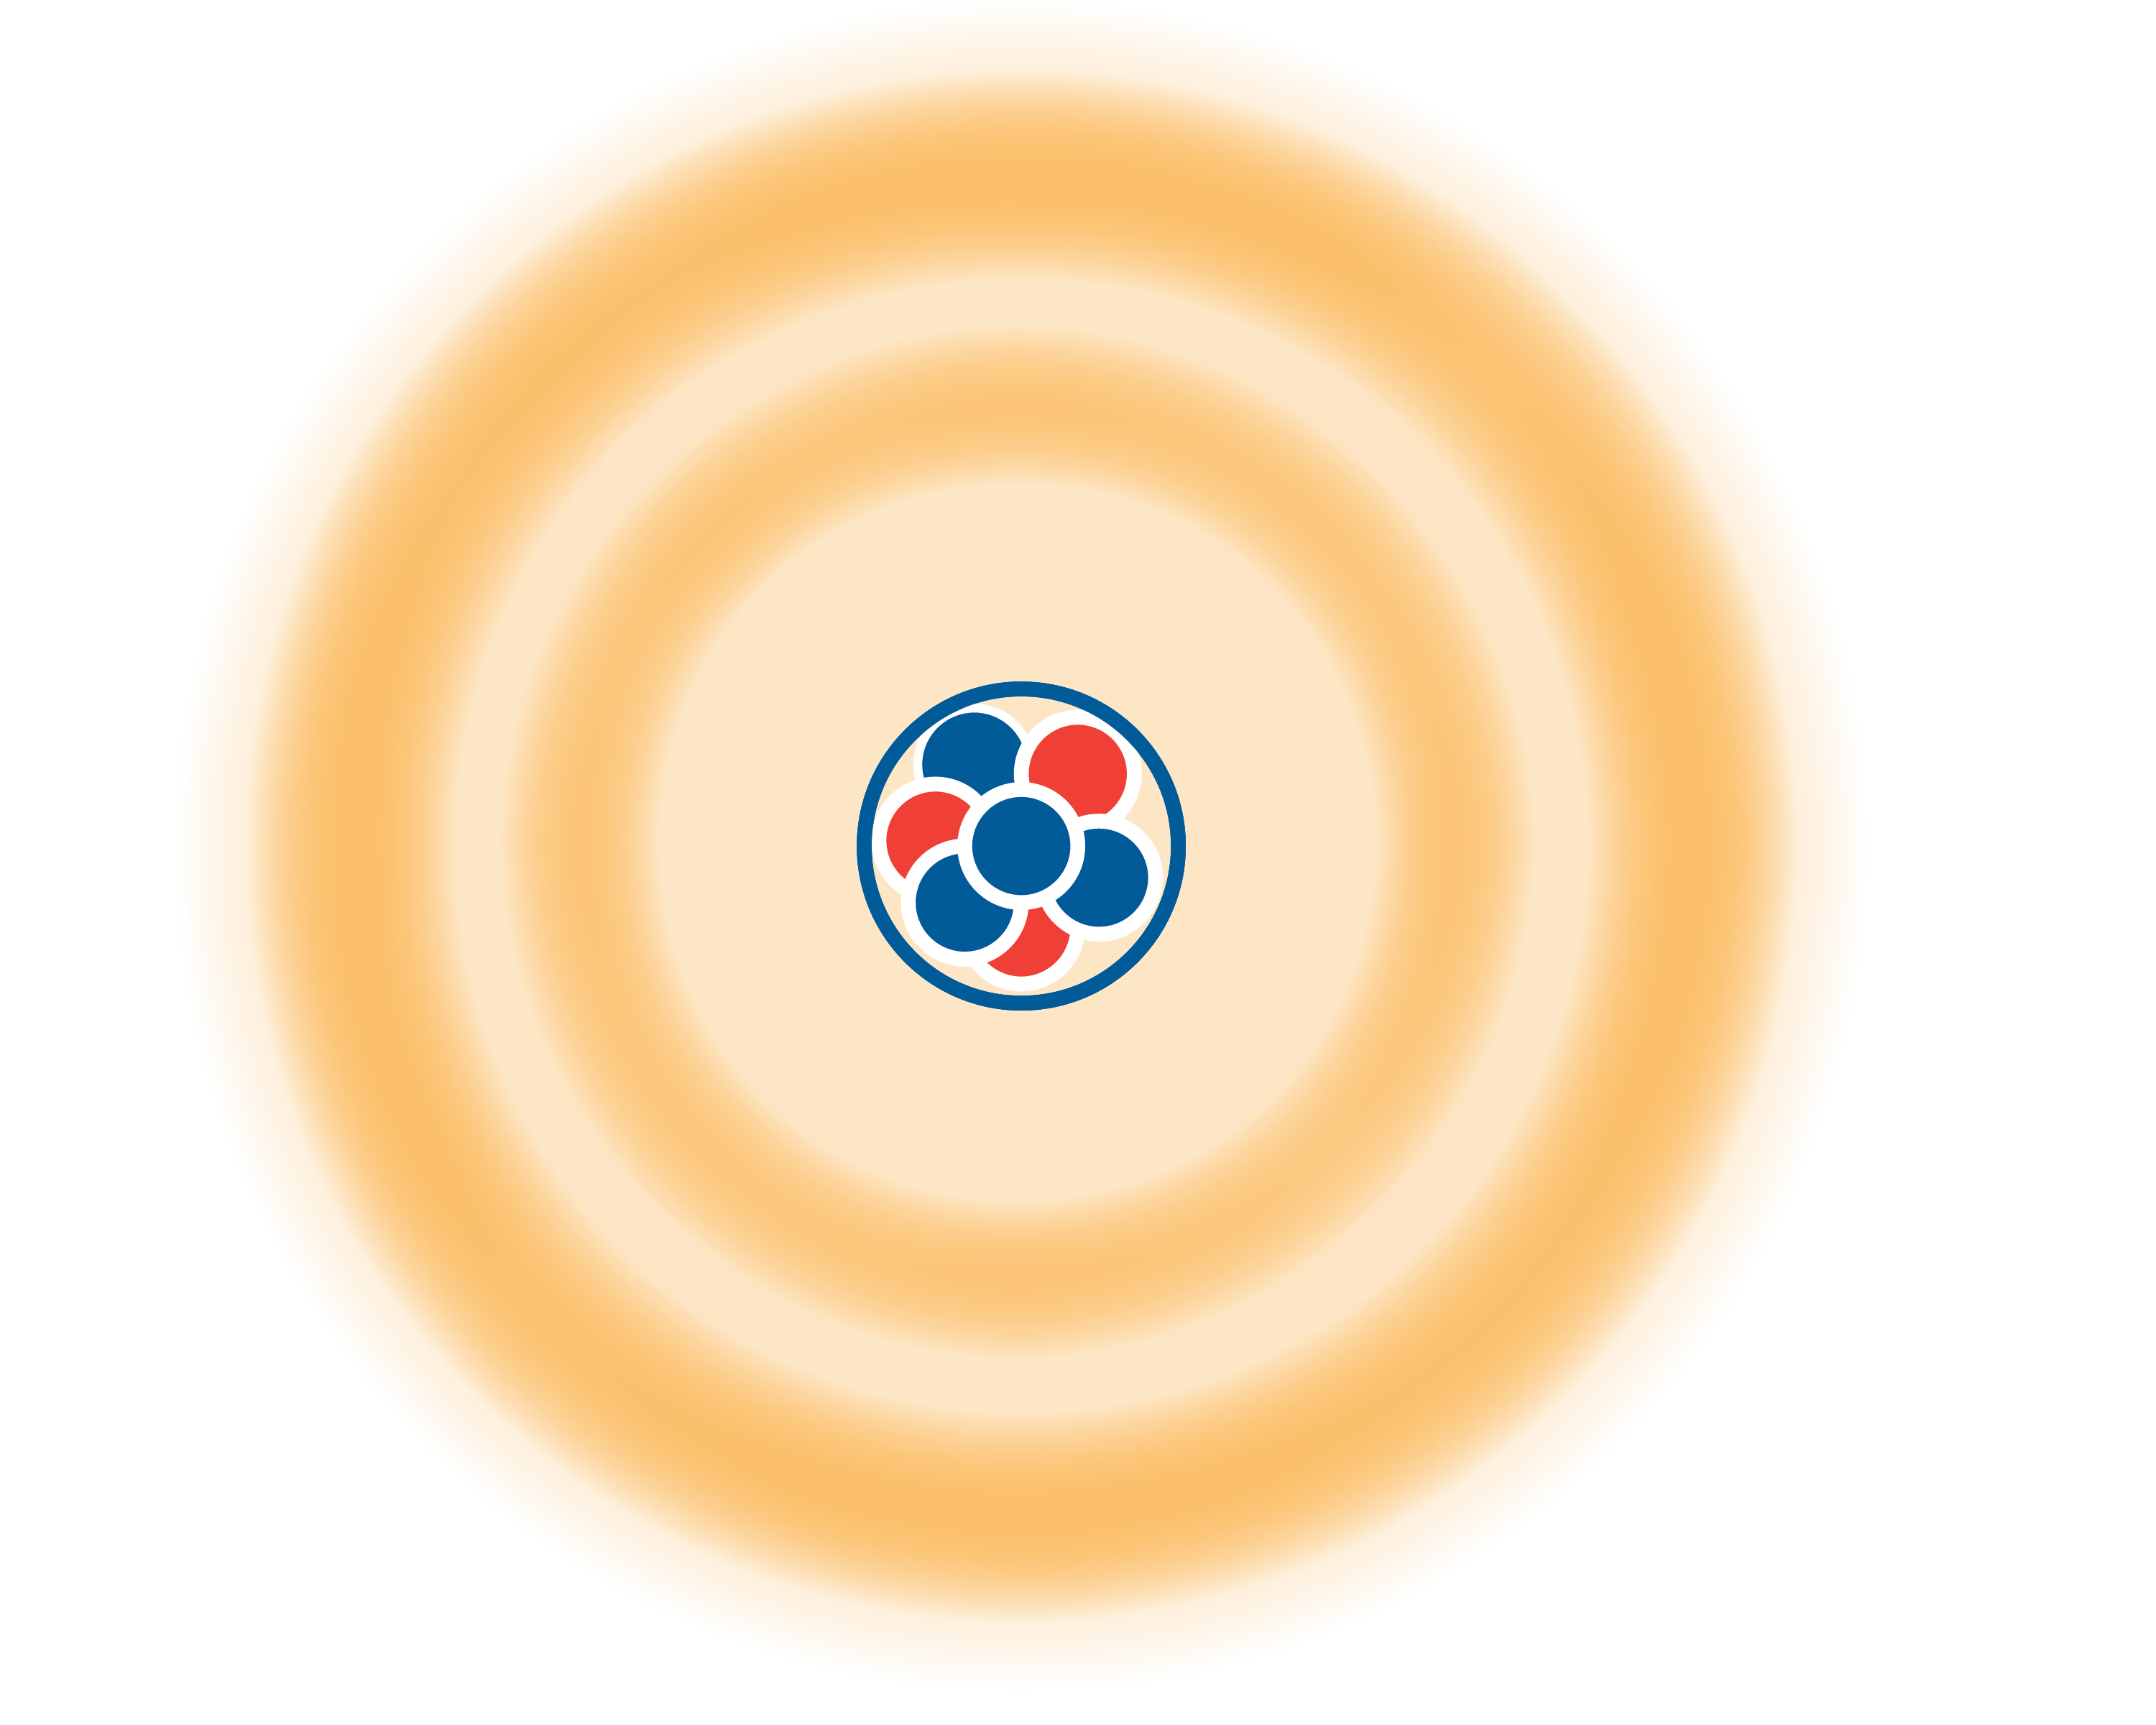
\includegraphics[trim={0 5cm 0 0}, width=3in]{atomCloud.png}
\end{wrapfigure}


We classify atoms by the numbers of protons they have. An atom with one proton is a
hydrogen atom, an atom with two protons is a helium atom, and so forth (refer to periodic table on pg..). We say that hydrogen and helium are \textit{elements} because the classification of elements is based on proton number. And we give
each element an atomic symbol. Hydrogen gets $H$. Helium gets $He$ Oxygen gets
$O$. Carbon gets $C$\index{elements}, etc.

Often two hydrogen atoms will attach to an oxygen atom. The result is
a water molecule. Why do they cluster together? because they share
electrons in their clouds.\index{molecules}
% ADD:Electronegativity

A molecule is described by the elements it contains. Water is $H_2O$
because it has two hydrogen atoms and one oxygen atom.

There are many kinds of molecules. You know a few:
\begin{itemize}
\item Table salt is crystals made of $NaCl$ molecules: a sodium atom attached to a chlorine atom.
\item Baking soda, or sodium bicarbonate, is $NaHCO_3$.
\item Vinegar is a solution including acetic acid ($CH_3COOH$).
\item $O_2$ is the oxygen molecules that you breathe out of the air (Air, a blend of gases, is mostly $N_2$.).
\end{itemize}

\subsection{Reading the Periodic Table}
The Periodic Table organizes what we know about the structure of different
elements. Each element has its own block or tile on the Periodic Table, and the
information on the tile tells us about the structure of that atom. Take a look at
the tile for carbon: (FIXME add carbon tile)

There are two key numbers: the atomic number and the average atomic mass. The
atomic number tells how many protons there are in the nucleus of any atom of
carbon. All carbon atoms have 6 protons. The other number is the average atomic
mass. Have you heard of carbon-14 dating? The phrase "carbon-14" refers to a rare
type of carbon that decays radioactively. By seeing how much carbon-14 has
decayed, scientists can estimate the age of organic materials, such as bone or
ash. Carbon-14 is a radioactive isotope (or version) of carbon. The 14 refers to
the mass number - the total amount of protons AND neutrons in the nucleus. The
most common isotope of carbon is carbon-12, with 6 protons and 6 neutrons in its
nucleus. Carbon-14, on the other hand, has 8 neutrons, which makes the nucleus
unstable, leading to radioactive decay. FIXME tow models comparing the structure
of  C-12 and C-14. FIXME resource: atom builder PhET. The average atomic mass is
the weighted average of all the carbon atoms in existence. Since the vast
majority of carbon is carbon-12, the average atomic mass is very close to 12. You
cannot determine the mass number of an individual atom from the periodic table:
it only tells you the average of all the isotopes. However, especially for light
atoms (atoms in the first two rows of the periodic table), you can usually
determine the mass number of the most common isotope by rounding the average
atomic mass to the nearest whole number.

\section{Chemical Reaction}

Sometimes two hydrogen atoms form a molecule ($H_2$). Sometimes two
oxygen atoms form a molecule ($O_2$). If you mix these
together and light a match, they will rearrange themselves into water
molecules. This is called a \textit{chemical reaction}.  In any
chemical reaction, the atoms are rearranged into new molecules.\index{chemical reaction}
% ADD: electronegativity

Some chemical reactions (like the burning of hydrogen gas described
above) are \textit{exothermic} -- that is, they give off energy.
Burning hydrogen gas happens quickly and gives off a lot of energy. If
you have enough, it will make quite an explosion.\index{exothermic}
% ADD: endo/ exo thermic graphs/ explanation

Other chemical reactions are \textit{endothermic} -- that is they consume
energy.  Photosynthesis, the process by which plants consume energy
from the sun to make sugar from $CO_2$ and $H_2O$ requires an endothermic
chemical reaction.\index{endothermic}


\section{Mass and Acceleration}

Each atom has a mass, so everything that is made up of atoms has a
mass, which is pretty much everything.  We measure mass in grams.  A
paper clip is about 1 gram of steel. An adult human can weigh 70,000
grams, so for larger things we often talk about kilograms. A kilogram
is 1000 grams.

The first interesting thing about mass is that objects with more mass
require more force to accelerate. For example, pushing a bicycle so
that it accelerates from a standstill to jogging speed in 2 seconds
requires a lot less force than pushing a train so that it accelerates
at the same rate.


\begin{mdframed}[style=important, frametitle={Newton's Second Law of Motion}]

The force necessary to accelerate an object of mass $m$ is given by:

$$F = m a$$

That is the force is equal to the mass times the acceleration.

\end{mdframed}

What are the units here? We already know that mass is measured in
kilograms. We can measure velocity in meters per second, but that is
different from acceleration. Acceleration is the rate of change in
velocity. So if we want to go from 0 to 5 meters per second (that's
jogging speed) in two seconds. That is a change in velocity of 2.5
meters per second every second. We would say this acceleration is $2.5
m/s^2$.

What about measuring force? Newton decided to name the unit after
himself: The force necessary to accelerate one kilogram at $1 m/s^2$
is known as \textit{a newton}. It is often denoted by the symbol $N$

\begin{Exercise}[title={Acceleration}, label=acceleration_train]

While driving a bulldozer, you come across a train car (with no brakes
and no locomotive) on a track in the middle of a city. The train car
has a label telling you that it weighs 2,400 kg. There is a bomb
welded to the interior of the train car, and the timer tells you that
you can safely push the train car for 120 seconds. To get the train
car to where it can explode safely, you need to accelerate it to 20 meters per
second. Fortunately, the track is level and the train car's wheels have
almost no rolling resistance.

With what force, in newtons, do you need to push the train for those 120 seconds?

\end{Exercise}
\begin{Answer}[ref=acceleration_train]
To get the train to 20 meters per second in 120 seconds, you must
accelerate it with a constant rate of $\frac{1}{6} m/s^2$. You
remember that $F = m a$, so $F = 2400 \times \frac{1}{6}$. Thus, you
will push the train with a force of 400 newtons for the 120 seconds
before the bomb goes off.
\end{Answer}

\section{Mass and Gravity}

The second interesting thing about mass is that masses are
attracted to each other by the force we call \textit{gravity}. The
force of attraction between two objects is proportional to the product
of their masses, and inversely proportional to their distance squared.
Meaning as objects get farther away, the force decreases.
That is why you are more attracted to the earth than you are to
distant stars, which have much more mass than the earth.
%ADD: Collums Law

\begin{mdframed}[style=important, frametitle={Newton's Law of Universal Gravitation}]

Two masses ($m_1$ and $m_2$) that are a distance of
$r$ from each other, are attracted toward each other with a force of
magnitude:

$$F = G\frac{m_1 m_2}{r^2}$$

where $G$ is the universal gravitational constant. If you measure the
mass in kilograms and the distance in meters. $G$ is about $6.674
\times 10^{-11}$.  That will get you the force of the attraction in
newtons.

\end{mdframed}

\begin{Exercise}[title={Gravity}, label=gravity_earth]

  The earth's mass is about $6 \times 10^{24}$ kilograms.

  Your spacecraft's mass is 6,800 kilograms.

  Your spacecraft is also about 100,000 km from the center of the earth. (For reference, the moon is about 400,000 km from the center of the earth.)

  What is the force of gravity that is pulling your spacecraft and the earth toward each other?

\end{Exercise}
\begin{Answer}[ref=gravity_earth]

  $$F = G\frac{m_1 m_2}{r^2} = (6.674 \times 10^{-11})\frac{(6.8 \time 10^3)(6 \times 10^{24})}{(10^5)^2} = 6.1 \times 10^{6}$$

  About 6 million newtons.

\end{Answer}

\section{Mass and Weight}

Gravity pulls on things proportional to their mass, so we often
ignore the difference between mass and weight.

The weight of an object is the force due to the object's mass and
gravity.  When we say, ``This potato weighs 1 pound,'' we actually mean
``This potato weighs 1 pound on earth.''  That same potato would weigh
about one-fifth of a pound on the moon.

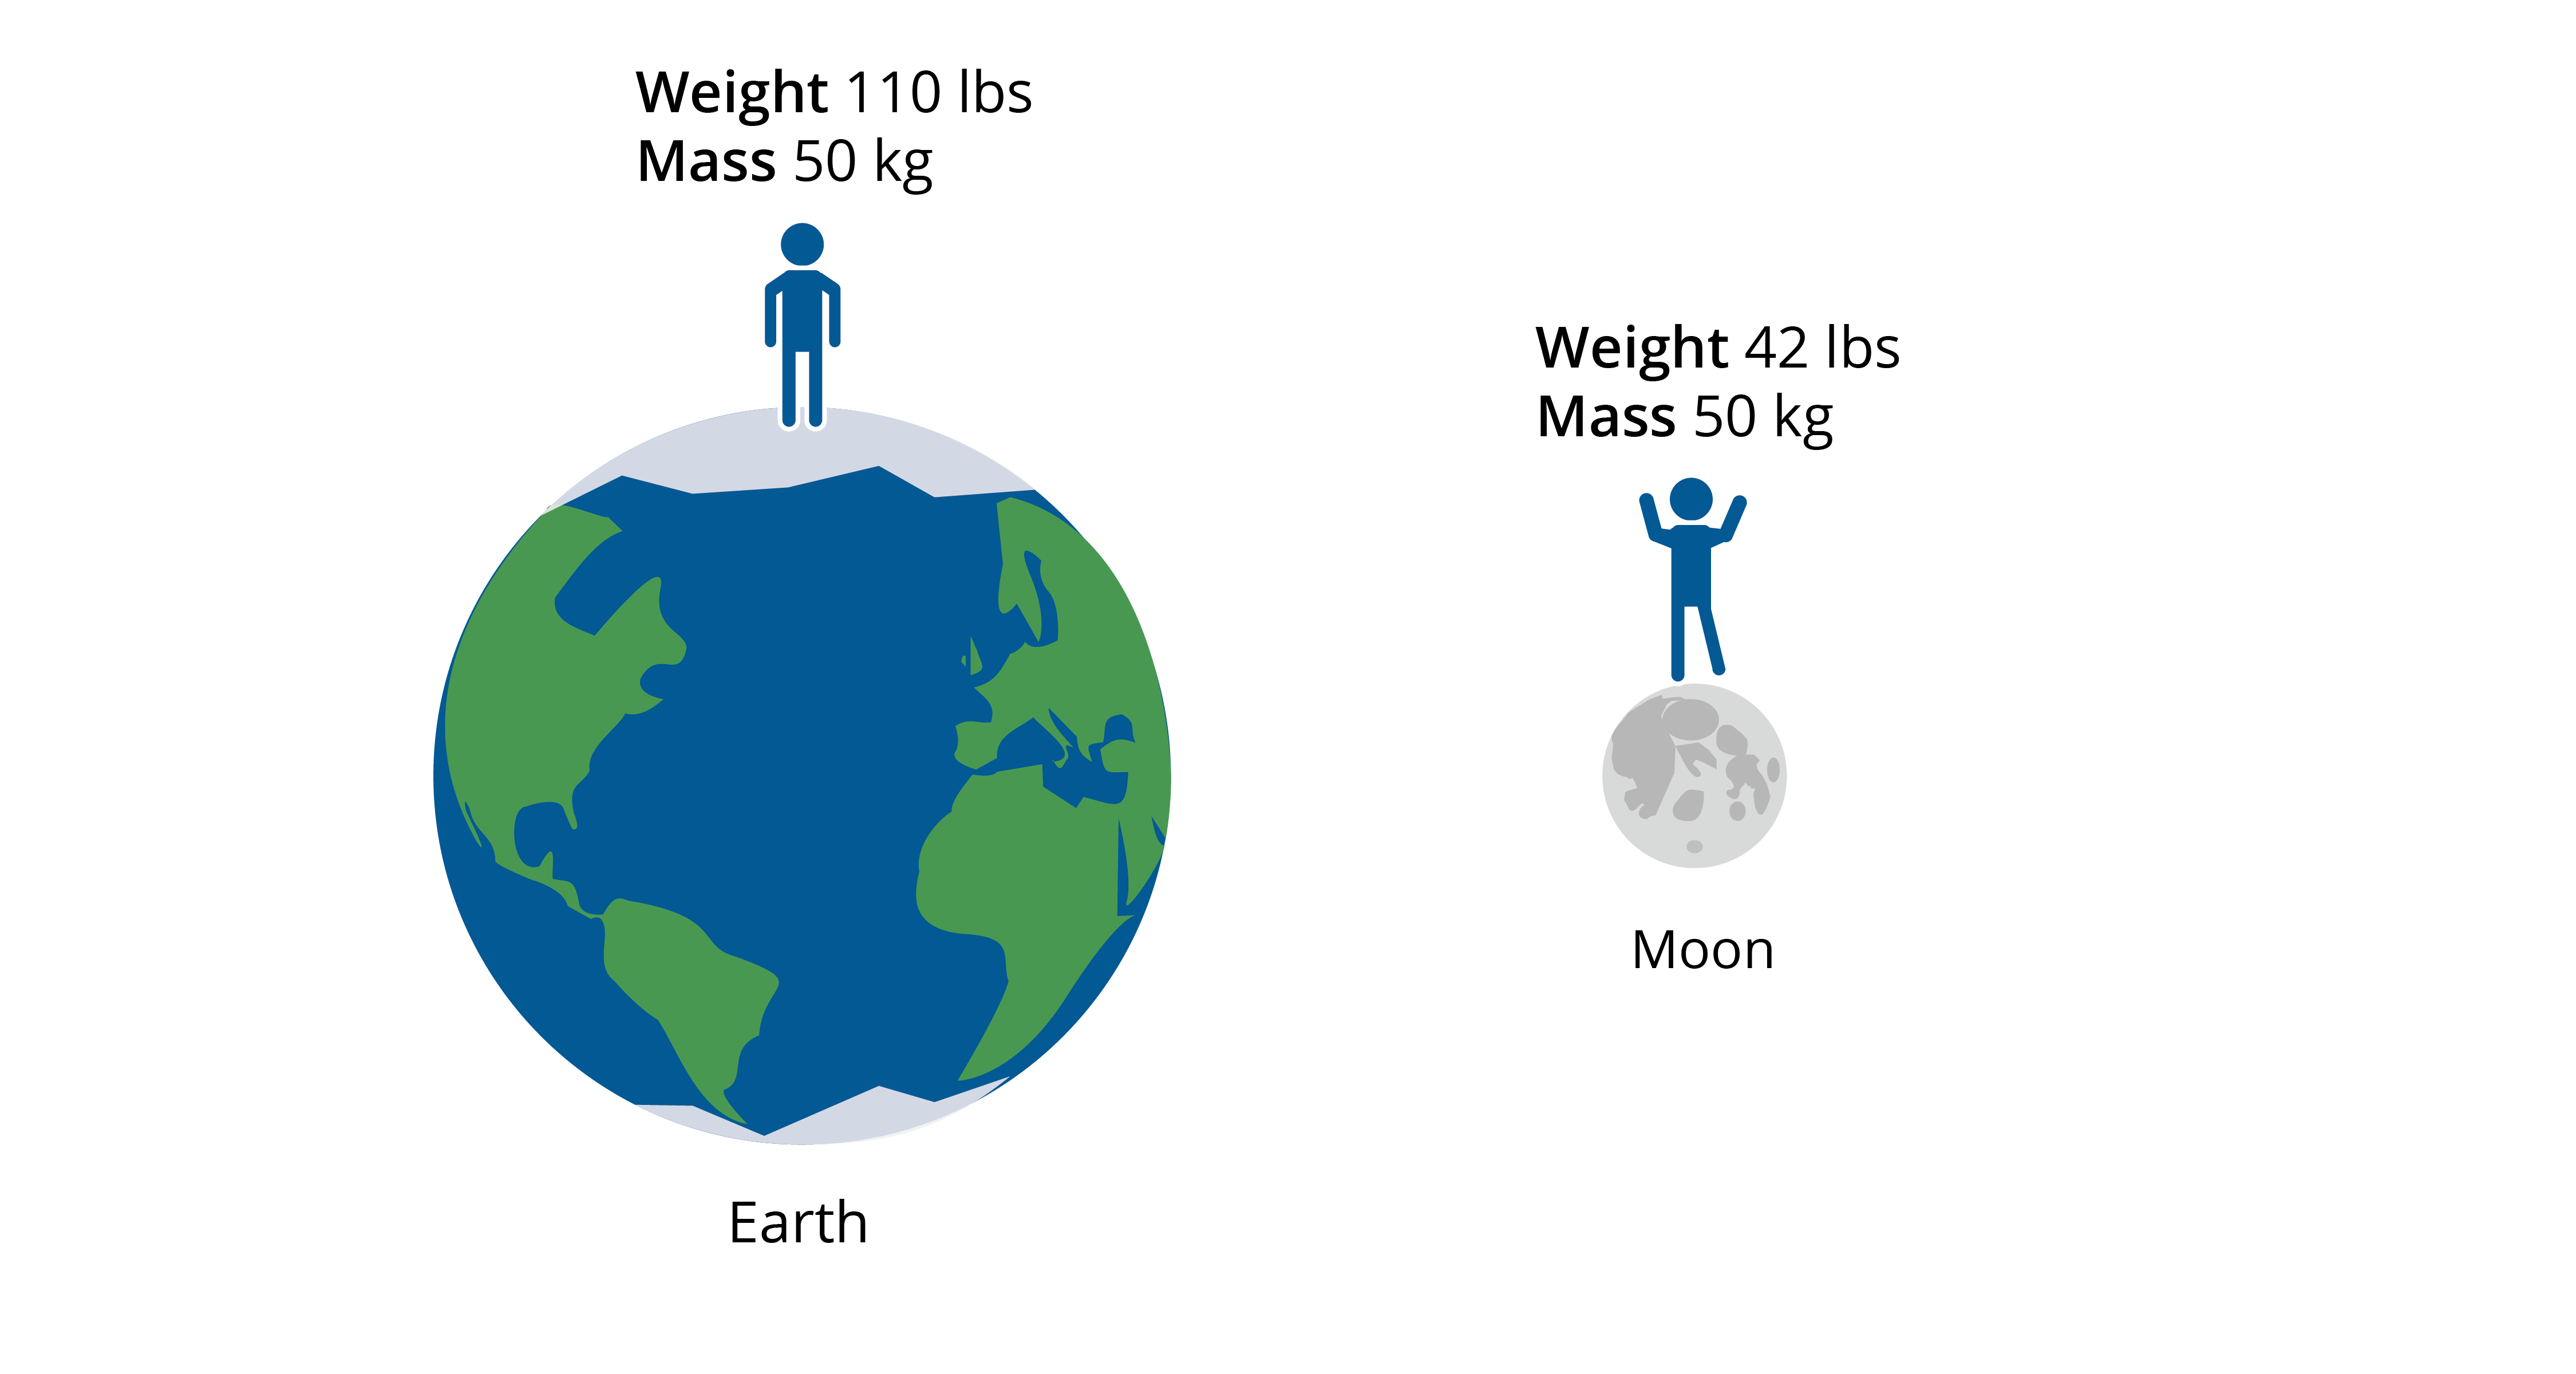
\includegraphics[width=0.7\textwidth]{massvweight.png}

But that potato has a mass of 0.45 kg anywhere in the universe.

FIXME Global layout note: Let's discuss adding Title's and Captions to all graphics.\\

For example:\\
TITLE: Mass versus Weight\\
CAPTION: Human Earth weight: 150lbs / Moon weight:??lbs\\
Potato Earth weight: .25lbs / Moon weight: ??lbs \\

FIXME:
Allison thinks it would be funny if the person in the graphic were holding a potato and we also added the weight and mass of the  potato to the caption. No worries if this type of edit isn't in the budget!

FIXME: What are your thoughts about using the metric system consistently -- in which case we'll replace pounds here with kilos. Max notes: we should explicitly use kilos for mass and pounds or newtons for weight. Kilos are a scalar measure of the amount of matter and pounds are a vector force of gravity on a particular piece of matter. Many students struggle to differentiate between mass and weight at a theoretical level due to casual comparison between pounds and kilos.
